En esta sección se explicarán con detalle algunos aspectos del comportamiento del sistema.  Concretamente se explicará cómo funciona el proceso de importación de datos, el framework de soporte a las visualizaciones y la llamada a las plantillas de la sección de datos.


\subsection{Proceso de importación de datos}
A continuación se detallarán los pasos del proceso de importación de datos al portal.  Tal y como se ha explicado en la ``\nameref{vista_sistema}'' éste proceso es realizado por el Punto de Entrada de Datos o \textit{Receiver}.  La arquitectura de dicho componente puede verse con detalle en la sección ``\nameref{vista_receiver}'' del presente capítulo.

La figura \ref{fig:diagrama_actividad_receiver} muestra el diagrama de actividad del proceso de importación de datos.  Los pasos de dicho proceso son los siguientes:
\begin{enumerate}
	\item El Punto de Entrada de Datos o \textit{Receiver} recibe una petición de inserción de datos por parte de algún importador.
	\item En primer lugar el Punto de Entrada de Datos comprueba si el verbo utilizado por la petición es un verbo correcto.  Concretamente el único verbo HTTP aceptado es POST.  En caso de que la petición utilizara un verbo distinto de POST, el Punto de Entrada de Datos envía una respuesta con código de error HTTP 405\footnote{El código de error HTTP 405 tiene el significado ``\textit{Method Not Allowed}''.  Para más información a cerca de los códigos de estado HTTP véase la especificación del W3C al respecto, \cite{w3c:http-status-codes}}.
	\item Posteriormente el Punto de Entrada de Datos comprueba si la dirección IP de la que procede la petición está en la lista blanca de direcciones admitidas para la importación de datos.  En caso de que la dirección IP de origen no se encontrara en la lista blanca, el Punto de Entrada de Datos envía una respuesta con un código de error HTTP 403\footnote{El código de error 405 tiene el significado ``\textit{Forbidden}''.  Para más información a cerca de los códigos de estado HTTP véase la especificación del W3C al respecto, \cite{w3c:http-status-codes}}.
	\item Tras comprobar que la petición utiliza un verbo correcto y procede de una fuente confiable, el Punto de Entrada de Datos comprueba que también incluye todos los parámetros necesarios.  En caso de que la petición no incluyera todos los parámetros, el Punto de Entrada de Datos responde con un código de error HTTP 400\footnote{El código de error 4005 tiene el significado ``\textit{Bad Request}''.  Para más información a cerca de los códigos de estado HTTP véase la especificación del W3C al respecto, \cite{w3c:http-status-codes}}.
	\item Una vez que las todas las validaciones han sido realizadas con éxito, se procede a la ejecución de los servicios de persistencia de datos.
		\begin{enumerate}
			\item En primer lugar se ejecuta el servicio de persistencia SQL, el cual almacena los datos provenientes de la petición en la base de datos MySQL.
			\item Posteriormente se ejecuta el servicio de persistencia RDF, que almacena los datos en el servidor semántico (como se ha explicado en la sección ``\nameref{chapter02:alternativas_seleccionadas}'' del capítulo \ref{chapter02} el servidor semántico seleccionado ha sido Virtuoso).
			\item Por último se ejecuta el servicio de persistencia de CKAN, que almacena la información en el catálogo de datos (tal y como se ha explicado anteriormente en la sección ``\nameref{chapter02:alternativas_seleccionadas}'' del capítulo \ref{chapter02} el catálogo de datos seleccionado ha sido CKAN.).
		\end{enumerate}
	\item En ultimo lugar y tras haber ejecutado todos los servicios de persistencia, el Punto de Entrada de Datos finaliza el proceso enviando una respuesta HTTP 200 e indicando que todo ha funcionado correctamente.
\end{enumerate}

\begin{figure}[ht]
	\centering
	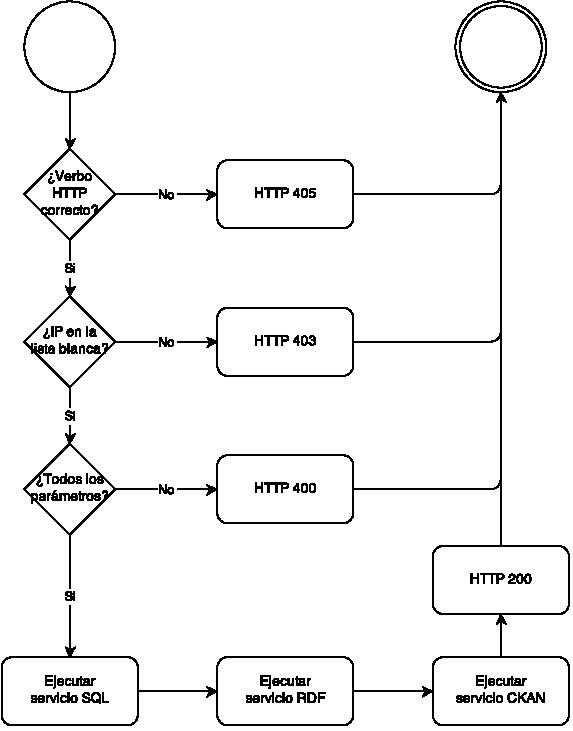
\includegraphics[width=\textwidth]{actividad/actividad_receiver}
	\caption{Diagrama de actividad del proceso de importación de datos}
	\label{fig:diagrama_actividad_receiver}
\end{figure}


\subsection{Funcionamiento del framework de soporte a visualizaciones}


\subsection{Llamada a las plantillas de la sección de datos}